\chapter{Fondamenti di Calcolo delle Probabilità e Statistica}
In questo Capitolo verranno riportate alcune nozioni base di Probabilità e Statistica applicabili nel campo della simulazione informatica, indispensabili per la costruzione e l’uso di
modelli di simulazione stocastica.

\section{Variabili stocastiche}
Un modello di simulazione è un modello intrinsecamente stocastico. Infatti i valori usati per le variabili di ingresso, di stato iniziale e i parametri sono decisi a partire dal sistema reale attraverso delle misurazioni fisiche, ogni valore appartiene a una distribuzione di probabilità. Perciò abbiamo bisogno di ripassare alcune nozioni base della probabilità in modo da comprendere i valori estratti da queste distribuzioni.\\

Una variabile stocastica o aleatoria $x_i$ rappresenta l'uscita di un'attività casuale. Essa può assumere n differenti valori dato $i ={1,2,...,n}$, ciascuno con una determinata probabilità $p_i(x) = p_1,p_2,...,p_n$.\label{fun_prob} L'insieme di tutte le probabilità è detto \textbf{funzione discreta di probabilità}. Da ricordare che la somma di tutte le singole probabilità da come risultato 1, ovvero:
\[ \sum_{i=1}^{n} p_i(x) = 1\]

\noindent Esse possono essere definite anche nel seguente modo.\\
Uno spazio di probabilità è una tripla $(\Omega, \mathcal{F}, P)$ dove:
\begin{itemize}
    \item $\Omega$ è lo spazio campione, il quale è un insieme di elementi (spesso l'insieme dei possibili esiti);
    \item $\mathcal{F}$ è lo spazio degli eventi, il quale è una famiglia di sottoinsiemi di $\Omega$ che ha le seguenti proprietà:
    \begin{enumerate}
        \item  $\Omega \in \mathcal{F} $,
        \item $A \in \mathcal{F} \Rightarrow \Omega \setminus A \in \mathcal{F}$,
        \item $A,B \in \mathcal{F} \Rightarrow A \cup B \in \mathcal{F} $.
    \end{enumerate}
    \item $P: \mathcal{F} \rightarrow [0,1]$ è la funzione di probabilità (definita come $p(x)$ in \ref{fun_prob}), la quale è una funzione reale con la seguenti proprietà:
    \begin{enumerate}
        \item $P(A) \geq  0 ,\forall \in \mathcal{F}$,
        \item $P(\Omega) = 1$,
        \item $(A, B \in \mathcal{F}) \wedge(A \cap B=\emptyset) \Longrightarrow P(A \cup B)=P(A)+P(B)$.
    \end{enumerate}
\end{itemize}

Dato uno spazio di probabilità, una variabile casuale è una funzione $ X : \Omega \rightarrow \Re$ che ha la seguente proprietà, per ogni reale $r$, $\{\omega \in \Omega: X(\omega) \leq r\} \in \mathcal{F}$. La funzione $F_X(x) = P(X \leq x = P( \{\omega \in \Omega: X(\omega) \leq r\})$, definita sull'insieme dei reali, è detta \textbf{funzione di distribuzione}.
Le variabili stocastiche o casuali vengono utilizzate poiché nei sistemi da simulare spesso si presentano degli eventi non facilmente prevedibili a priori, come ad esempio l'arrivo di clienti ad uno sportello o la quantità di pioggia in una determinata stagione. Perciò tali fenomeni vengono rappresentati tramite queste variabili dalle quali estrarne poi la distribuzione di probabilità.

\paragraph{Esempio} Si consideri il numero di pazienti che si presentano ad un
ambulatorio tra le 9 e le 10 di mattina, e poniamo $\Omega = {0, 1, 2, . . .}$, $\mathcal{F}= 2^\Omega$ ,
e $X(\omega) = \omega$ (la funzione identità). La funzione X così definita è una variabile
casuale, infatti, per ogni reale $r$ è
\[ \{\omega \in \Omega: X(\omega) \leq r\} = \{0,...,\left \lfloor r \right \rfloor\} \in \mathcal{F}\]


\subsection{Funzione densità di probabilità}
La \textbf{funzione densità di probabilità $f(x)$} si utilizza per definire la probabilità di una variabile di assumere uno specifico valore tra infiniti valori , la quale è praticamente nulla, a causa del processo osservato che è continuo. Detto ciò essa si può definire come la probabilità che $ x_1 \leq x \leq x_2$, ovvero che il valore di x sia compreso in intervallo $[x_1, x_2]$, data da:
\begin{align*}
     & p(x_1 \leq x \leq x_2) = \int_{x_1}^{x_2}f(x) d(x)= \\
     &  \int_{-\infty }^{+ \infty} f(x) dx = 1
\end{align*}
   
\subsection{Funzione cumulativa di distribuzione}
La \textbf{funzione cumulativa di distribuzione $F(x)$} definisce la probabilità che un certo valore sia minore o uguale a x, la quale si può descrivere come:
\[ F(x) = \int_{- \infty}^{X}f(x) d(x) \]
Da cui risulta che $0 \leq F(x) \leq 1$ e $p( x_1 \leq x \leq x_2) = F(x_2) - F(x_1)$.

\subsection{Media}
Per una variabile discreta \footnote{Una variabile casuale è detta \textbf{discreta} se l'insieme di valori che può assumere è numerabile.} si definisce il \textbf{valore atteso} o \textbf{media $E(x)$ oppure $\mu_x$} come:
\[ E(x) =  \sum_{i=1}^{n} x_i p_i(x)\]
Si definisce media di una funzione $y=g(x)$:
\[ E(g(x)) = \sum_{i=1}^{n} g(x_i) p_i(x)\]
Per una variabile continua si ha che la media è pari a:
\[ E(x) = \int_{-\infty}^{+ \infty} xf(x)dx = \lambda_1 = \lambda\]
e per una funzione continua y:
\[ E(x) = \int_{-\infty}^{+ \infty} g(x)f(x)dx = \int_{-\infty}^{+ \infty} g(x)dF(x)\]

Altro...

\subsection{Varianza}
Si definisce \textbf{varianza} di x e si indica con $\sigma^2(x)$, è la media degli scarti quadratici rispetto alla media $\mu_x$ e rappresenta una misura di dispersione di x. La sua radice quadrata, $\sigma_x$ è detta \textbf{deviazione standard}. La varianza è definita come 
\[ \sigma^2(x) = E(x-\lambda)^2 = \int_{-\infty}^{+\infty}(x-\lambda)^2 f(x)dx  \]
Da cui si ricava facilmente
\[\sigma^2(x) = E(x^2) - E^2(x)\]
Se x è una \textbf{variabile discreta} si ha
\[ \sigma^2(x) = \sum_{i=1}^{n}(x_i -E(x))^2 \cdot p_i(x)\]
La deviazione standard viene definita come
\[ \sigma(x) = \sqrt{\sigma^2(x)}\]
\subsubsection{Teorema di Beniaymé-Chebychev}
Il Teorema di Beniaymé-Chebychev lega la deviazione standard di x alla probabilità di deviazione dei singoli valori di x della media:
\[ p(\left | x- \lambda \right | \geq k\sigma) \leq \frac{1}{k^2}   \]
 Ovvero, qualunque sia la forma di $f(x)$, la probabilità al di fuori di $\pm k \sigma$ è limitata, $\leq \frac{1}{k^2}$.
 
 \subsection{Funzione di probabilità di due variabili aleatorie} \label{subsec:prob_congiunta}
 In modo analogo al precedente si definisce la funzione di distribuzione $F(X,Y)$ di due variabili aleatorie x e y
 \[ F(X,Y) = p(x \leq X, y \leq Y)\]
 che indica la probabilità che $x \leq X$ ,valore prefissato, e $y \leq Y$. La suddetta funzione è detta anche \textbf{funzione di probabilità congiunta} e scritta $F(x,y)$.
 Da essa possiamo ottenere la definizione di \textbf{densità congiunta di probabilità}. Nel caso di variabili discrete data l'esistenza di un insieme numerabile di punti 
 \[ (X_1, Y_1), (X_1,Y_2),...,(X_2,Y_2),...,(X_i,Y_j)\]
 con associati numeri positivi 
 \[\ p_{11},p_{12},...,p_{21},p_{22},...,p_{ij}\]
\noindent i quali soddisfano la relazione $F(X_h, Y_k) = \sum_{i}^{}\sum_{j}^{}p_{ij}$ con $\sum_{i}^{}\sum_{j}^{}p_{ij}=1$ sommata per tutti gli i e j per i quali $X_i \leq X_h$ e $Y_j \leq Y_k$.
Allora si può definire $p = (x=X_i, y=Y_j) = p_{ij}$ per tutti gli i e j per i quali esistono dei valori delle variabili x e y, assumendo $p_{ij} = 0$ altrove. Quindi la \textbf{funzione discreta di probabilità congiunta} è $f(x_i, y_j) = p_{ij}$ con distribuzione cumulativa $F(x_i,y_j)$.\\
Se invece la funzione F(x,y) è continua si definisce la \textbf{densità congiunta}
\[f(x,y) = \dfrac{\lambda}{\lambda x} \dfrac{\lambda}{\lambda y} F(x,y) \] e quindi
\[F(x,y) = \int_{-\infty}^{y}\int_{-\infty}^{x} f(x,y) dxdy\]
\[ p(a \leq x\leq b , c \leq y \leq d) = \int_{c}^{d}\int_{a}^{b} f(x,y) dxdy \]
\[ p( X \leq x \leq X + dX , Y \leq y \leq Y +dY) = F(X,Y) dXdY\]

\subsection{Distribuzione marginale}
Si vuole determinare la probabilità g(x) e h(y) di una variabile x o y, data la densità congiunta f(x,y) di due. In poche parole la \textbf{distribuzione marginale} di un sottoinsieme di una collezione di variabili casuali è la distribuzione di probabilità delle variabili contenute nel sottoinsieme. Ciò si interpreta dicendo che si vuole la $p(x \leq X, $con y qualunque$)$ simboleggiata con $F(x, \infty)$ o $F(\infty,y)$.
Nel caso discreto si ha 
\[F(x_h, \infty) = \sum_{i}^{}\sum_{j}^{}p_{ij}\] 
Nel caso continuo si ha invece 
\[ F(x,\infty)=\sum_{-\infty}^{X} \sum_{-\infty}^{\infty} f(x,y) dxdy= \int_{-\infty}^{X} g(x) dx \]
Da cui si ha 
\[g(x) = \int_{-\infty}^{\infty}f(x,y) dy \]
\[h(y) = \int_{-\infty}^{\infty}f(x,y) dx \]

dove g(x) e h(y) sono dette \textbf{distribuzioni marginali} di x e y.

\subsection{Indipendenza}
Due variabili aleatorie x e y sono dette \textbf{indipendenti} se , detta f(x,y) la loro densità congiunta e g(x) e h(y) le relative distribuzioni marginali si ha:
\[ f(x,y) = g(x) \cdot h(y)\]
La condizione necessaria e sufficiente alla validità della formula sopra è che f(x,y) può essere fattorizzata nel prodotto di due funzioni, ovvero:
\[f(x,y) = r(x) \cdot s(y)\]

\subsection{Variabili completamente dipendenti e variabili stocasticamente correlate}
Per coppie di variabili dipendenti si ha che f(x,y)=g(x)=h(y), ovvero la probabilità f(x,y) è uguale a 0 solo per coppie x,y dove y è una funzione ad un solo valore di x e viceversa.
In tutti i casi in cui f(x,y) non è né il prodotto $g(x) \cdot h(y)$ né tale che g(x)=h(y)=f(x,y) le variabili x e y si dicono stocasticamente correlate.
Il coefficiente di correlazione misura il grado di correlazione il quale è pari a:
\begin{itemize}
    \item 0 se e solo se $f(x,y) = g(x) \cdot h(y)$
    \item $|1|$ se e solo se $f(x,y)=g(x)=h(y)$
    \item $0\leq |x| \leq 1$ in tutti gli altri casi.
\end{itemize}

\subsection{Probabilità condizionali}
La \textbf{probabilità condizionale} identifica la probabilità che una variabile x assuma il valore $x_i$, assunto che y assuma il valore $y_j$ si scrive:
\[p(x=x_i|y=y_j) = \dfrac{p(x=x_i,y=y_j)}{p(y=y_j}= \dfrac{f(x_i,y_j)}{h(y_j)}= g(x_i|y_j)\]
Si possono scrivere le funzioni densità condizionali di probabilità di x dato y e di y dato x:

 \begin{align*}
     g(x|y) =\dfrac{f(x,y)}{h(y)} \\
     h(y|x) = \dfrac{f(x,y)}{g(x)}
 \end{align*}
 
 Nel caso di variabili indipendenti di ha:
 \begin{align*}
     g(x|y) =g(x) \\
     h(y|x) = h(y)
 \end{align*}
 \subsection{Covarianza}
 La covarianza è una misura della relazione tra due variabili x e y, essa viene definita come di seguito:
 \[cov(x,y) = E(xy) - E(x)E(y)\]
 Dalla definizione risulta che:
\begin{itemize}
    \item cov(x,y)>0 se, nella funzione f(x,y) grandi valori di x sono associati a grandi valori di y e viceversa;
    \item cov(x,y)<0 se piccoli valori di x sono associati a grandi valori di y e viceversa;
    \item cov(x,y)=0 se, quando x è grande, alcuni valori di y sono grandi e alcuni piccoli.
\end{itemize}

\subsection{Coefficiente di correlazione}
Il \textbf{coefficiente di correlazione} p(x,y) tra due variabili si definisce come la misura standardizzata della covarianza e si scrive come:
\[p(x,y) = \dfrac{cov(x,y)}{\sigma(x) \sigma(y)}\]
Esso misura il grado di dipendenza lineare tra x e y. Il suo valore è compreso tra (-1,1), raggiungendo $\pm 1$ quando esiste una dipendenza perfettamente lineare tra x e y. Al contrario se x e y sono indipendenti allora si ha p=0, ma il contrario non è necessariamente vero. Questo vuol dire che se due variabili hanno p=0 sono dette \textbf{non correlate}, ma non è detto che siano indipendenti. Perciò l'uso di p come misura dell'indipendenza deve essere limitato a quei problemi che hanno una possibile dipendenza lineare.




\section{Generazione di numeri casuali}

\subsection{Metodo congruente lineare}
Il \textbf{metodo congruente lineare} serve per generare sequenze di interi compresi tra 0 e m da utilizzare per la generazione di distribuzioni uniformi, gli obiettivi da soddisfare sono:
\begin{enumerate}
    \item massimo periodo;
    \item granularità fine;
    \item efficienza di calcolo.
\end{enumerate}
Questo metodo usa la seguente funzione:
\[X_{i+1}=(aX_i + c) \text{mod m}\]
se c=0 il metodo di chiama \textbf{congruente moltiplicativo}.
La scelta dei parametri a= moltiplicatore e c= incremento è critica nel determinare il periodo e le doti di casualità. La funzione \verb|rand()| implementa il metodo congruente moltiplicativo con parametri $m= 2^31 -1 $ e $a=75$.

\subsection{Test del Chi-quadro $X^2$}
Per verificare le doti di casualità di una sequenza occorre sottoporla ad una serie di test:
\begin{itemize}
    \item Test del $X^2$
    \item Test seriale
    \item Test del gap
\end{itemize}
L'obiettivo di questi test è di verificare l'uniformità della distribuzione generata e la mancanza di correlazione tra numeri che si trovano ad una certa distanza k nella sequenza.
Per verificare l'uniformità si calcola:
\[V= \sum_{s=1}^{k}\dfrac{(Y_s - np_s)^2}{np_s}\]
Poi si confronta il valore ottenuto con la tabella dei percentili.
Il test del $X^2$ funziona nel seguente modo:
\begin{itemize}
    \item si dividono i possibili valori in k categorie;
    \item si genera un campione di n numeri e si contano le occorrenze di valori in ciascuna categoria $Y_s$;
    \item si calcola il valore atteso di valori in ciascuna categoria con la formula $p_s \cdot n$ dove $p_s$ è la probabilità di estrarre un valore nella categoria s;
    \item infine si calcola la sommatoria $V= \sum_{s=1}^{k}\dfrac{(Y_s - np_s)^2}{np_s}$.
\end{itemize}

\begin{figure}[H]
	\centering
    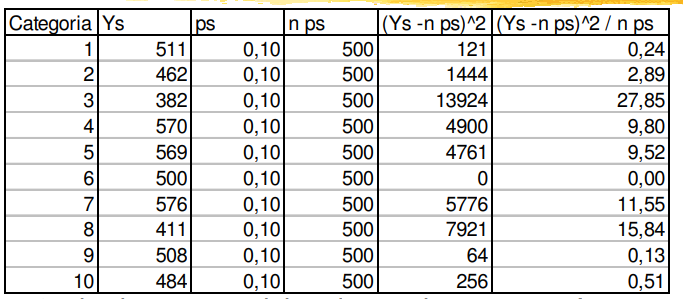
\includegraphics[width=15cm, keepaspectratio]{img/test_chi_quadro.png}
	\caption{Test del Chi-quadro.}\label{fig:chi_quadro}
\end{figure}

\subsection{Test per la verifica delle proprietà di casualità}
I valori $m= 2^31-1$, a=1 e c=1 garantiscono il periodo massimo e l'uniformità di distribuzione dei risultati ma non garantiscono l'assenza di correlazione fra i valori, per rilevare questo problema il test del $X^2$ può essere applicato a coppie di valori estratti dalla sequenza. Nell'esempio di prima si potrebbe dividere il range di valori in 5 sotto-range e formare 25 categorie corrispondenti a tutte le possibili coppie di sotto-range e la $p_s$ si calcola come prodotto delle probabilità di generare un valore in ciascuno di essi. Altri test sono quello del \textbf{gap} ovvero si calcola la lunghezza di sequenze i cui valori sono compresi tra $\alpha$ e $\beta$ e si confronta la loro distribuzione con quella teorica usando il chi-quadro.

\section{Generazione di distribuzioni qualsiasi}
Per la generazione di diverse distribuzioni si utilizzano i seguenti metodi:
\begin{itemize}
    \item\textbf{ Metodo della trasformazione inversa}
    \item \textbf{Metodo del rifiuto}
    \item \textbf{Metodo della composizione}
\end{itemize}

\subsection{Metodo della trasformazione inversa}
\begin{figure}[H]
	\centering
    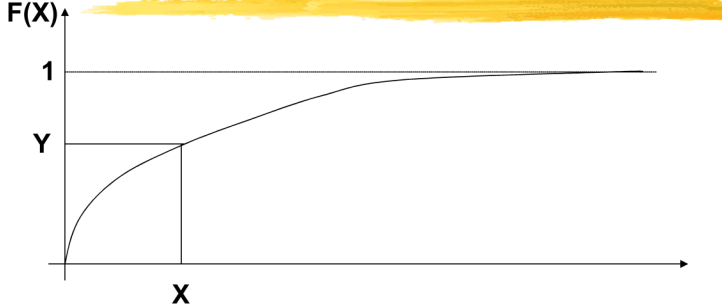
\includegraphics[width=15cm, keepaspectratio]{img/trasformazione_inversa.png}
	\caption{Trasformazione inversa.}\label{fig:trasformazione_inversa}
\end{figure}
Un esempio di applicazione del metodo è la generazione di variabili
casuali distribuite secondo una esponenziale negativa:
\begin{align*}
    & F(x) = 1 - e^{-\mu x} \\
    & 1-y = e^{- \mu x} \\
    & ln(1-y) = ln(e^{-\mu x}) = -\mu x\\
    & x = \dfrac{- ln(1-y)}{\mu}\\ 
\end{align*}
Se y è distribuita come U(0,1), anche Z = 1-Y ha la stessa distribuzione: quindi si può generare una sequenza distribuita secondo una esponenziale negativa semplicemente generando una sequenza con distribuzione U(0,1), applicando la funzione logaritmo naturale, cambiando di segno e dividendo per µ i numeri di tale sequenza.

\subsection{Metodo del rifiuto}
Quando non è facilmente ricavabile l'inversa della cumulativa si utilizzano altri metodi come il metodo del rifiuto.
\begin{figure}[H]
	\centering
    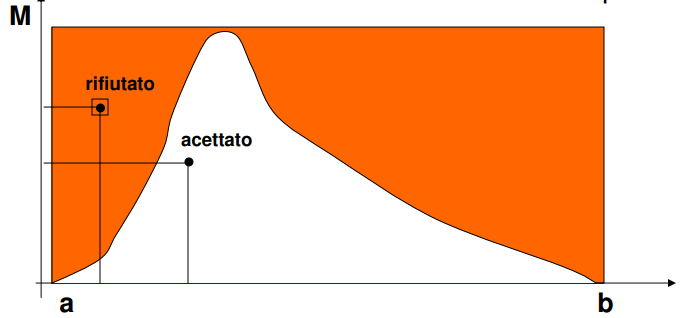
\includegraphics[width=15cm, keepaspectratio]{img/metodo_rifiuto.png}
	\caption{Metodo del rifiuto.}\label{fig:metodo_rifiuto}
\end{figure}
Si genera un valore y distribuito come U(0,M) e un x uniformemente distribuito tra a e b, se $y \leq f(x)$ allora si accetta x come valore generato della distribuzione, sennò si ripete con altri due valori di x e y.

\subsection{Metodo della composizione}
Questa distribuzione può essere vista come risultato della composizione di 4 uniformi: $U(a_1,a_2), U(a_2,a_3), U(a_3,a_4), U(a_4,a_5)$.
\begin{figure}[H]
	\centering
    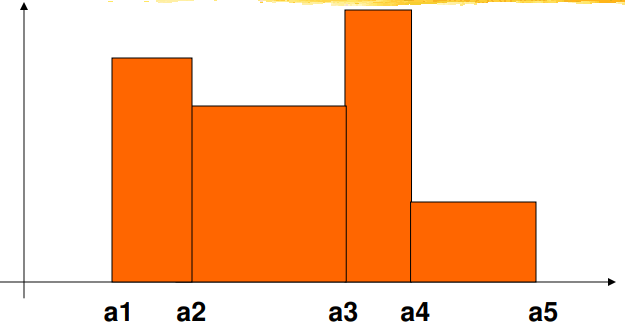
\includegraphics[width=15cm, keepaspectratio]{img/metodo_composizione.png}
	\caption{Metodo della composizione.}\label{fig:metodo_composizione}
\end{figure}
Siano $p_1, p_2, p_3$ e $p_4$ le aree dei quattro rettangoli: per generare un valore tratto da questa distribuzione scegliamo un rettangolo utilizzando le $p_i$, poi generiamo un numero uniformemente distribuito in $U(a_i, a_{i+1})$.

\section{Distribuzioni}